% TODO: Was originally after preface of APIs
\graphicspath{{mainmatter/background/figures/}}

\section{On the Development, Documentation and Usage of Web APIs}
\label{ssec:background:api:usage}

The development of web \glspl{api} (commonly referred to as a \textit{web service}) and web \glspl{api} traces its roots back to the early 1990s, where  the Open Software Foundation's \gls{dce} introduced a collection of services and tools for developing and maintaining distributed systems using a client/server architecture \citep{Rosenberry:1992up}. This framework used the synchronous communication paradigm \glspl{rpc} first introduced by \citet{Nelson:1981ue} that allows procedures to be called in a remote address space as if it were local. Its communication paradigm, \gls{dce}/\gls{rpc} \citep{OpenSoftwareFoundation:1991vp}, enables developers to write distributed software with underlying network code abstracted away. To bridge remote \gls{dce}/\glspl{rpc} over components of different operating systems and languages, an \gls{idl} document served as the common service contract or \textit{service interface} for software components. 

This important leap toward language-agnostic distributed programming paved way for \glsac{xml}-\gls{rpc}, enabling \glspl{rpc} over \glsac{http} (and thus the Web) encoded using \glsac{xml} (instead of octet streams \citep{OpenSoftwareFoundation:1991vp}). As new functionality was introduced, this lead to the natural development of the \gls{soap}, the backbone messaging connector for \gls{ws} applications, a realisation of the \gls{soa} \citep{Casati:2003vi} pattern. The \gls{soa} pattern prescribes that services are offered by service providers and consumed by service consumers in a platform- and language-agnostic manner and are used in large-scale enterprise systems (e.g., banking, health). Key to the \gls{soa} pattern is that a service's quality attributes (see \cref{sec:background:software-quality}) can be specified and guaranteed using a \gls{sla} whereby the consumer and provider agree upon a set level of service, which in some cases are legally binding \citep{Bass:2003wi}. This agreement can be measured using \gls{qos} parameters met by the service provider during the transportation layer (e.g., response time, cost of leasing resources, reliability guarantees, system availability and trust/security assurance \citep{Hwang:2017tr,Weerawarana:2005wx}). These attributes are included within \gls{soap} headers; thus, \gls{qos} aspects are independent from the transport layer and instead exist at the application layer \citep{Pautasso2008}. The \gls{idl} of \gls{soap} is \gls{wsdl}, providing a description of how the web service is invoked, what parameters to expect, and what data structures are returned.

\begin{figure}[h!]
  \centering
  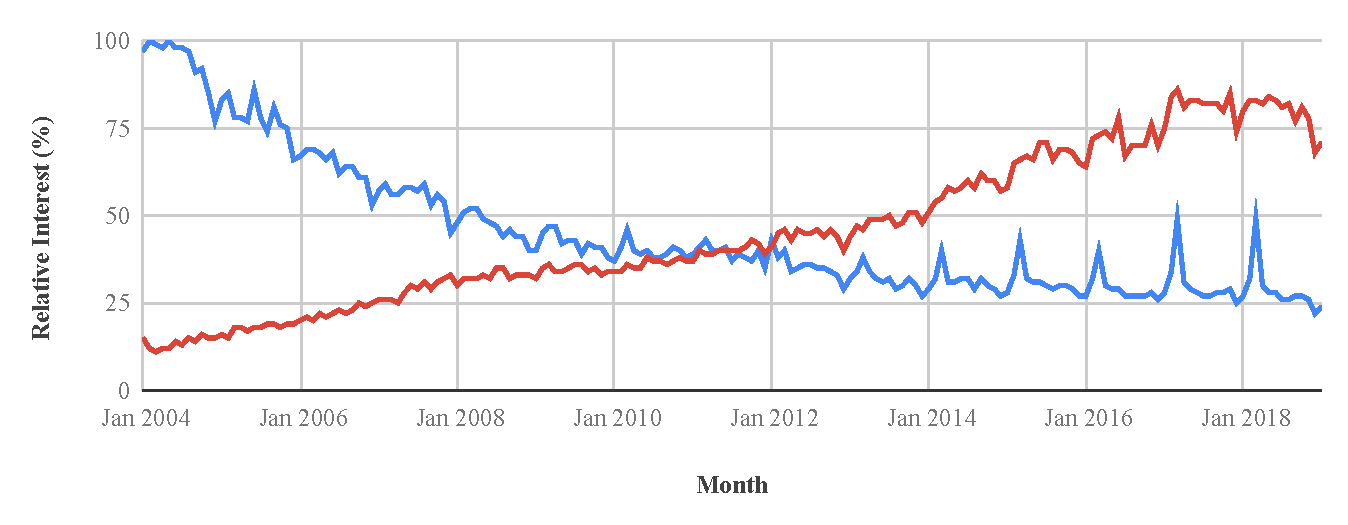
\includegraphics[width=\linewidth]{rest-vs-soap}
  \caption[SOAP versus REST search interest over time]{Worldwide search interest for \glsac{soap} (blue) and \glsac{rest} (red) since 2004. Source: Google Trends.}
  \label{fig:background:apis:rest-vs-soap}
\end{figure}

While it is rich in metadata and verbosity, discussions on whether this was a benefit or drawback came about the mid-2000s \citep{zurMuehlen:2005ci,Pautasso2008} whether the amount of data transfer paid off (especially for mobile clients where data usage was scarce). Developer usability for debugging the \gls{soap} `envelopes' (messages POSTed over \glsac{http} to the service provider component) was difficult, both due to the nature of \glsac{xml}'s wordiness and difficulty to test (by sending POST requests) in-browser. As a simple example, 25 lines (794 bytes) of \glsac{http} communication is transferred to request a customer's name from a record using \gls{soap} (\cref{lst:background:apis:soap-request,lst:background:apis:soap-response}). 

\begin{samepage}
\begin{lstlisting}[language=xml,label=lst:background:apis:soap-request,caption={[An example SOAP request]A \gls{soap} \glsac{http} POST consumer request to retrieve customer record \#43456 from a web service provider. Source: \citep{Ballinger:2014aa}.}]
POST /customers HTTP/1.1
Host: www.example.org
Content-Type: application/soap+xml; charset=utf-8

<?xml version="1.0"?>
<soap:Envelope 
  xmlns:soap="http://www.w3.org/2003/05/soap-envelope">
  <soap:Body>
    <m:GetCustomer 
      xmlns:m="http://www.example.org/customers">
      <m:CustomerId>43456</m:CustomerId>
    </m:GetCustomer>
  </soap:Body>
</soap:Envelope>
\end{lstlisting}
\begin{lstlisting}[language=xml,label=lst:background:apis:soap-response,caption={[An example SOAP response]The \gls{soap} \glsac{http} service provider response for \cref{lst:background:apis:soap-request}. Source: \citep{Ballinger:2014aa}.}]
HTTP/1.1 200 OK
Content-Type: application/soap+xml; charset=utf-8

<?xml version='1.0' ?>
<env:Envelope 
  xmlns:env="http://www.w3.org/2003/05/soap-envelope" >
  <env:Body>
    <m:GetCustomerResponse 
      xmlns:m="http://www.example.org/customers">
      <m:Customer>Foobar Quux, inc</m:Customer>
    </m:GetCustomerResponse>
  </env:Body>
</env:Envelope>
\end{lstlisting}
\end{samepage}

\gls{soap} uses the architectural principle that \glslongpl{ws} (or the applications they provide) should remain \textit{outside} the web, using \glsac{http} only as a tunnelling protocol to enable remote communication \citep{Pautasso2008}. That is, the \glsac{http} is considered as a transport protocol solely. In 2000, \citet{Fielding:2000vh} introduced \gls{rest}, which instead approaches the web as a medium to publish data (i.e., \glsac{http} is part of the \textit{application} layer instead). Hence, applications become amalgamated into of the Web. \citeauthor{Fielding:2000vh} bases \gls{rest} on four key principles:

\begin{itemize}
  \item \textbf{\glsacpl{uri} identify resources.} Resources and services have a consistent global address space that aides in their discovery via \glsacpl{uri} \citep{BernersLee:2004vf}.
  \item \textbf{\glsac{http} verbs manipulate those resources.} Resources are manipulated using the four consistent \glsac{crud} verbs provided by \glsac{http}: POST, GET, PUT, DELETE.
  \item \textbf{Self-descriptive messages.} Each request provides enough description and context for the server to process that message.
  \item \textbf{Resources are stateless.} Every interaction with a resource is stateless.
\end{itemize}

\noindent
Consider the equivalent example of \cref{lst:background:apis:soap-request,lst:background:apis:soap-response} but in a \glsac{rest}ful architecture (\cref{lst:background:apis:rest-request,lst:background:apis:rest-response}) and it is clear why this style has grown more popular with developers (as we highlight in \cref{fig:background:apis:rest-vs-soap}). Developers have since embraced \gls{rest}ful \gls{api} development, though the major drawback of \gls{rest}ful services is its lack of a uniform \gls{idl} to facilitate development (though it is possible to achieve this using \gls{wadl} \citep{Mandel:2008ww}).  Therefore, no RESTful service uses a standardised response document or invocation syntax. While there are proposals, such as \gls{wadl} \citep{Hadley:2006vv}, \glsac{raml}\footnoteurl{https://raml.org}{25 January 2019}, \gls{api} Blueprint\footnoteurl{https://apiblueprint.org}{25 January 2019}, and the OpenAPI\footnoteurl{https://www.openapis.org}{25 January 2019} specification (initially based on Swagger\footnoteurl{https://swagger.io}{25 January 2019}), there is still no consensus as there was for \gls{soap} and convergence of these \glspl{idl} is still underway.

\begin{samepage}
\begin{lstlisting}[label=lst:background:apis:rest-request,caption={[An example RESTful request]An equivalent \glsac{http} consumer request to that of \cref{lst:background:apis:soap-request}, but using \gls{rest}. Source: \citep{Ballinger:2014aa}.}]
GET /customers/43456 HTTP/1.1
Host: www.example.org
\end{lstlisting}
\begin{lstlisting}[language=json,label=lst:background:apis:rest-response,caption={[An example RESTful response]The \gls{rest} \glsac{http} service provider response for \cref{lst:background:apis:rest-request}.}]
HTTP/1.1 200 OK
Content-Type: application/json; charset=utf-8

{"Customer": "Foobar Quux, inc"}
\end{lstlisting}
\end{samepage}

%\cref{sec:background:probabilistic-stochastic} 
%For you to assign agency to a machine, the machine has to communicate back to you an assurance—that's how to frame it
%If you increasingly give it more agency, what is the two-way comms between user and machine look like?
%A way of doing assurances is the five-level automation framework of self-driving cars (see Simon's work RE this)
%What does the assurance packet look like? What do you think you should give to an engineer so that they trust you and give sufficient control to it? E.g., TCP/IP has a built-in pushback throttle; fewer ACK means it slows down packet sending as assurance is not given from client to server (adjust the rate of transmission)—use this as a metaphor
